% Created 2016-11-06 Sun 16:47
\documentclass[a4paper,12pt]{article}
\usepackage[utf8]{inputenc}
\usepackage[T1]{fontenc}
\usepackage{fixltx2e}
\usepackage{graphicx}
\usepackage{grffile}
\usepackage{longtable}
\usepackage{wrapfig}
\usepackage{rotating}
\usepackage[normalem]{ulem}
\usepackage{amsmath}
\usepackage{textcomp}
\usepackage{amssymb}
\usepackage{capt-of}
\usepackage{hyperref}
\usepackage{fullpage}
\usepackage[T1]{fontenc}
\usepackage[francais, frenchb]{babel}
\usepackage{lmodern}
\usepackage{authblk}
\author[]{Guillaume Denis\thanks{guillaume.denis3@etu.univ-lorraine.fr}}
\author[]{Geoffrey Gaillard\thanks{geoffrey.gaillard3@etu.univ-lorraine.fr}}
\affil{Université de Lorraine, UFR Mathématiques et Informatique}
\renewcommand\Authand{  et }
\hypersetup{
colorlinks,%
citecolor=black,%
filecolor=black,%
linkcolor=black,%
urlcolor=blue
}
\date{\today}
\title{Bibal \\ \small{Application de gestion de bibliothèque}}
\hypersetup{
 pdfauthor={Geoffrey Gaillard},
 pdftitle={Bibal \\ \small{Application de gestion de bibliothèque}},
 pdfkeywords={},
 pdfsubject={},
 pdfcreator={Emacs 24.5.1 (Org mode 8.3.6)},
 pdflang={Frenchb}}
\begin{document}

\vfill

\maketitle

\thispagestyle{empty}

\clearpage


\thispagestyle{empty}

\tableofcontents

\clearpage



\section{Analyse du cahier des charges}
\label{sec:orgheadline3}

\subsection{Rappel}
\label{sec:orgheadline1}

Bibal est une application de gestion de bibliothèque destinée à assurer le suivi
des ouvrages, des exemplaires, des auteurs, des usagers ainsi que leurs emprunts
et réservations. La bibliothèque possède deux types d’ouvrage: les livres et les
magazines. Les usagers n’ont accès qu'à la page d’accueil de l’application, où
ils peuvent consulter la liste des ouvrages de la bibliothèque. Ils doivent
passer par l’intermédiaire d’un bibliothécaire pour effectuer des réservations,
des emprunts ou consulter la disponibilité des exemplaires.

\subsection{L’analyse de la demande}
\label{sec:orgheadline2}



Nous avons discerné trois cas d’usage :
\begin{itemize}
\item gérer les usagers, c'est-à-dire les personnes consultant la bibliothèque dans le but d’utiliser ses services,
\item gérer les ouvrages et les exemplaires, c'est-à-dire toutes les ressources bibliographiques,
\item gérer les emprunts et les réservations, qui concerne les services proposés par la bibliothèque aux usagers.
\end{itemize}

Une œuvre représente soit un livre soit un magazine et est immatérielle. Elle
désigne bien l’œuvre et non un exemplaire d’un livre ou d’un magazine. Un
exemplaire est un livre physique ou un magazine physique. Un exemplaire peut
être emprunté, être réservé, être rendu, être abîmé. Un usager est un
utilisateur de l’application Bibal, qu’il soit employé de la bibliothèque ou
non. Une réservation concerne une œuvre et un usager. L’usager peut donc
réserver une œuvre, dès qu’un exemplaire de cette œuvre est disponible,
l’usager peut l’emprunter. Sa réservation devient alors un emprunt.\\



La gestion des usagers inclus:
\begin{itemize}
\item laisser la possibilité aux usagers sans droits de consulter les œuvres disponibles,
\item l’ajout, la modification et la suppression d’un usager,
\item l’affectation d’un usager à une réservation ou à un emprunt.
\end{itemize}

La gestion des ouvrages inclus:
\begin{itemize}
\item l’ajout, la modification et la suppression des œuvres et des exemplaires,
\item le suivi des nouvelles œuvres des auteurs,
\item le suivi des parutions des magazines.
\end{itemize}

La gestion des exemplaires et des réservations concerne:
\begin{itemize}
\item le suivi de l’état (en état, abîmé, etc.) des exemplaires,
\item le suivi du statut des exemplaires (emprunté, réservé, disponible).
\end{itemize}

\clearpage

\section{Modélisation de la solution}
\label{sec:orgheadline16}
\subsection{Les usages}
\label{sec:orgheadline6}

Voici, sous forme schématique, les trois cas d’usage que nous avons discerné:

\begin{figure}[htb]
\centering
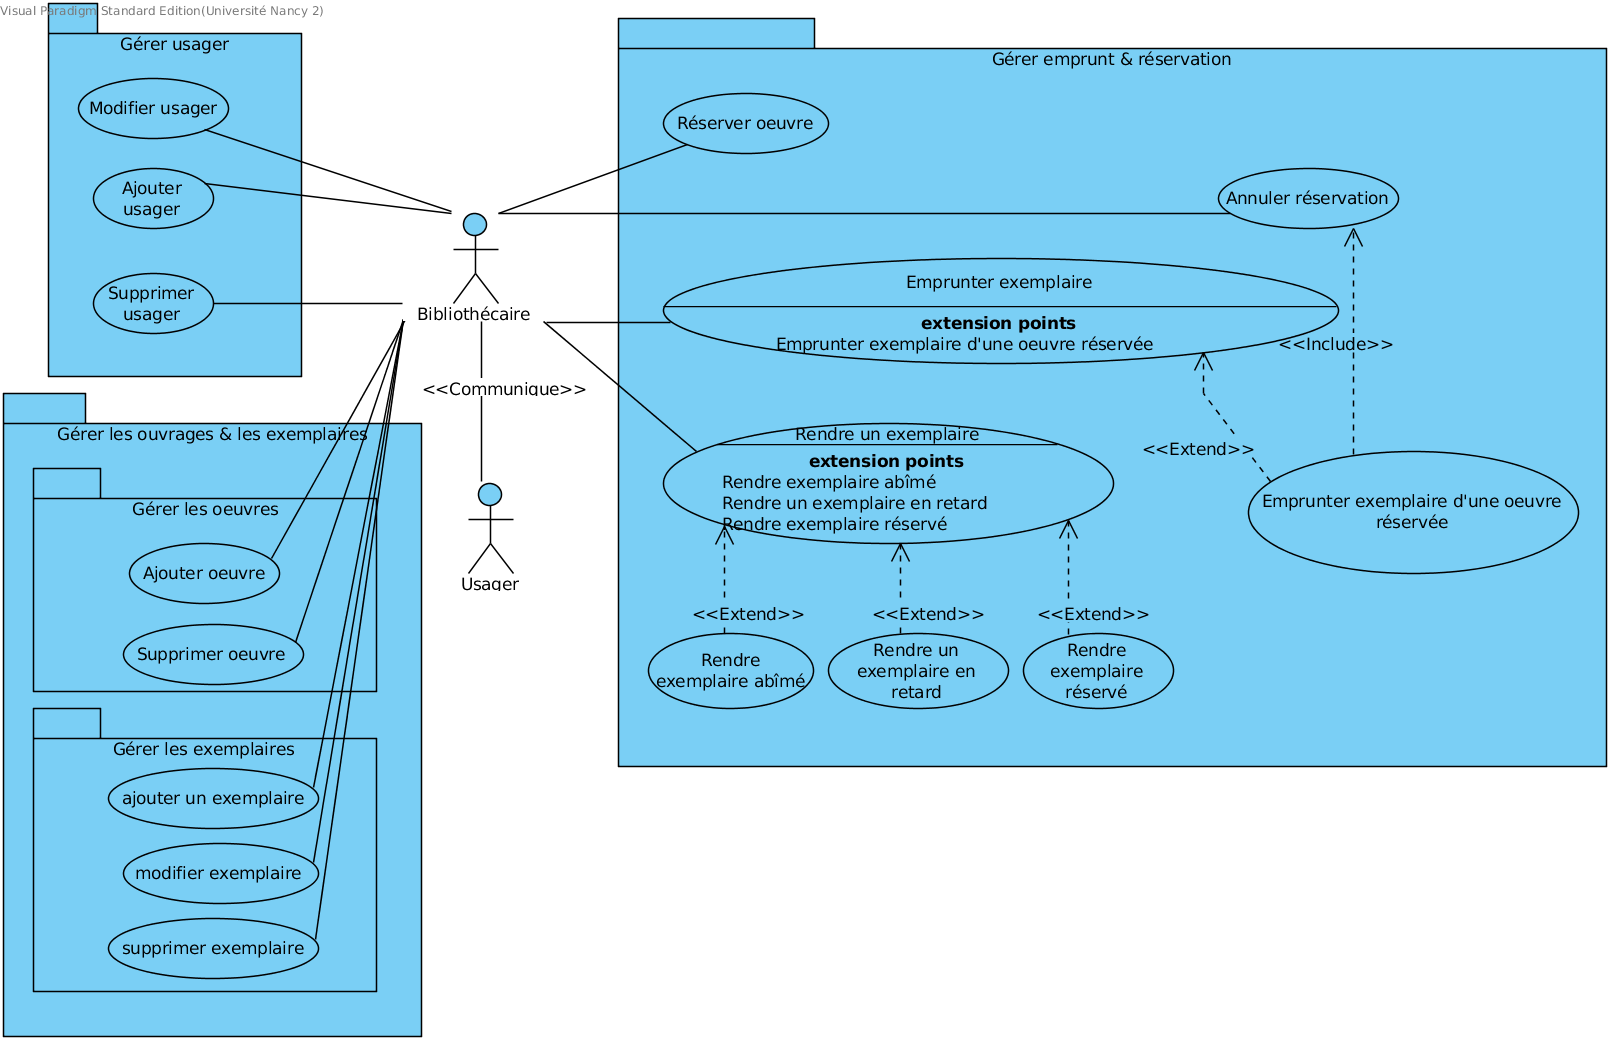
\includegraphics[width=.9\linewidth]{./res/img/cas-d-utilisation.png}
\caption{\label{fig:orgparagraph1}
Cas d'utilisation}
\end{figure}


On retrouve les trois pôles que qui ont été extraits suite à notre analyse du cahier des charges :
\begin{itemize}
\item gérer les usagers,
\item gérer les ouvrages et les exemplaires,
\item gérer les emprunts et les réservations.
\end{itemize}

Chaque pôle doit permettre d’effectuer les opérations basiques de lecture, création, modification et
suppression (on utilisera le l'acronyme CRUD pour désigner ces opérations).


Dans le cas des emprunts et des réservations un cas d’usage s’ajoute à ces
opérations basiques, rendre un exemplaire qui a été emprunté. Il est lui-même
décliné en trois cas d’utilisation en fonction de différents paramètres :
\begin{itemize}
\item rendu d’un exemplaire abîmé,
\item rendu d’un exemplaire après la date limite,
\item rendu d’un exemplaire réservé par un autre utilisateur.
\end{itemize}

Lors de l’implémentation de l’application, ces cas d’utilisation devront tous être réalisables.


Pour décrire plus finement les cas d’utilisation modélisés précédemment nous
avons utilisé des diagrammes d’activité. Cela nous a permis, pour chaque cas
d’utilisation, de définir les étapes à réaliser pour mener à bien ce cas. Nous
allons nous concentrer sur deux cas d’utilisation : réserver une œuvre et
emprunter un exemplaire d’une œuvre réservée.


\subsubsection{Réserver une œuvre}
\label{sec:orgheadline4}
\begin{figure}[htb]
\centering
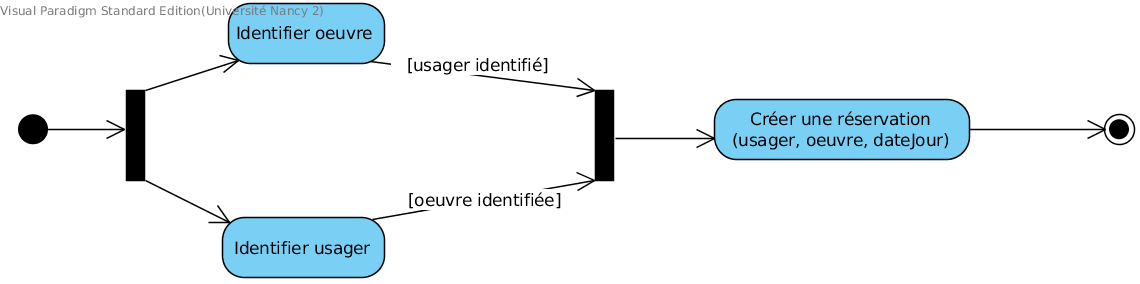
\includegraphics[width=.9\linewidth]{./res/img/reserver-oeuvre1.png}
\caption{\label{fig:orgparagraph2}
Réserver une œuvre}
\end{figure}

Le but de ce cas d’utilisation est la création d’une réservation pour
une œuvre donnée. Les étapes nécessaires et obligatoires à cette création
sont l’identification de l’œuvre en question et l’identification de l’usager
qui désire réserver l’œuvre. Il s’agit de la partie lecture des opérations
CRUD d’une œuvre et d’un usager.
Une fois les deux entités identifiées la bibliothécaire peut réserver une
œuvre au nom de l’usager datée du jour.

\clearpage

\subsubsection{Emprunter un exemplaire d’une œuvre réservée}
\label{sec:orgheadline5}

\begin{wrapfigure}[15]{r}{0.4\linewidth}

\label{wrap-fig:emprunt-reserve}
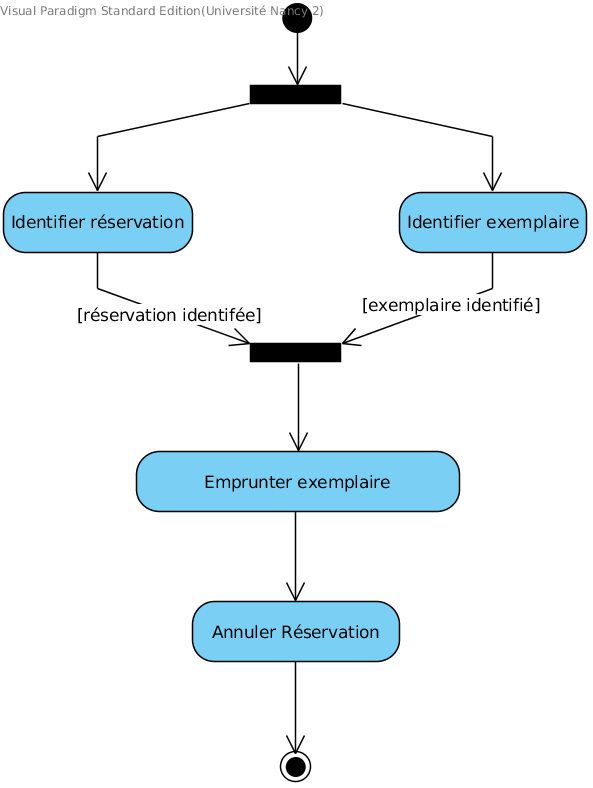
\includegraphics[width=\linewidth]{./res/img/emprunter-exemplaire-d-une-oeuvre-reservee.png}
\end{wrapfigure}


Ce cas d’utilisation annule une réservation effectuée par un usager lorsque
celui-ci parvient à emprunter un exemplaire de l’œuvre réservée.

Afin de parvenir à l’annulation effective de la réservation (équivalent à une suppression dans les opérations CRUD), la bibliothécaire doit passer par plusieurs étapes :

\begin{itemize}
\item Trouver la réservation émise sur l’œuvre concernée par l’usager concerné,
\item Trouver un exemplaire de cette œuvre qui n’est pas emprunté,
\item Créer un emprunt pour l’exemplaire par l’usager.
\end{itemize}


Les diagrammes pour les autres cas d’utilisation sont disponibles en annexe.

\subsection{Logique applicative}
\label{sec:orgheadline12}

Une fois la logique métier bien définie grâce aux cas d’utilisation et aux
diagrammes d’activité nous avons modélisé la logique applicative de la
solution au besoin exprimé dans le cahier des charges.

Dans un premier temps, un diagramme des classes nous a permis de définir les
objets métiers qui sont nécessaires à la réalisation de l’application. Pour les
cas induisant un changement d’état d’un objet métier, une modélisation à l’aide
d’un diagramme d’états a été choisie. Enfin, nous avons modélisé les
enchaînements de traitements effectués par l’application à l’aide de diagrammes
de séquence.

\clearpage

\subsubsection{Diagramme de classes}
\label{sec:orgheadline7}

\begin{figure}[htb]
\centering
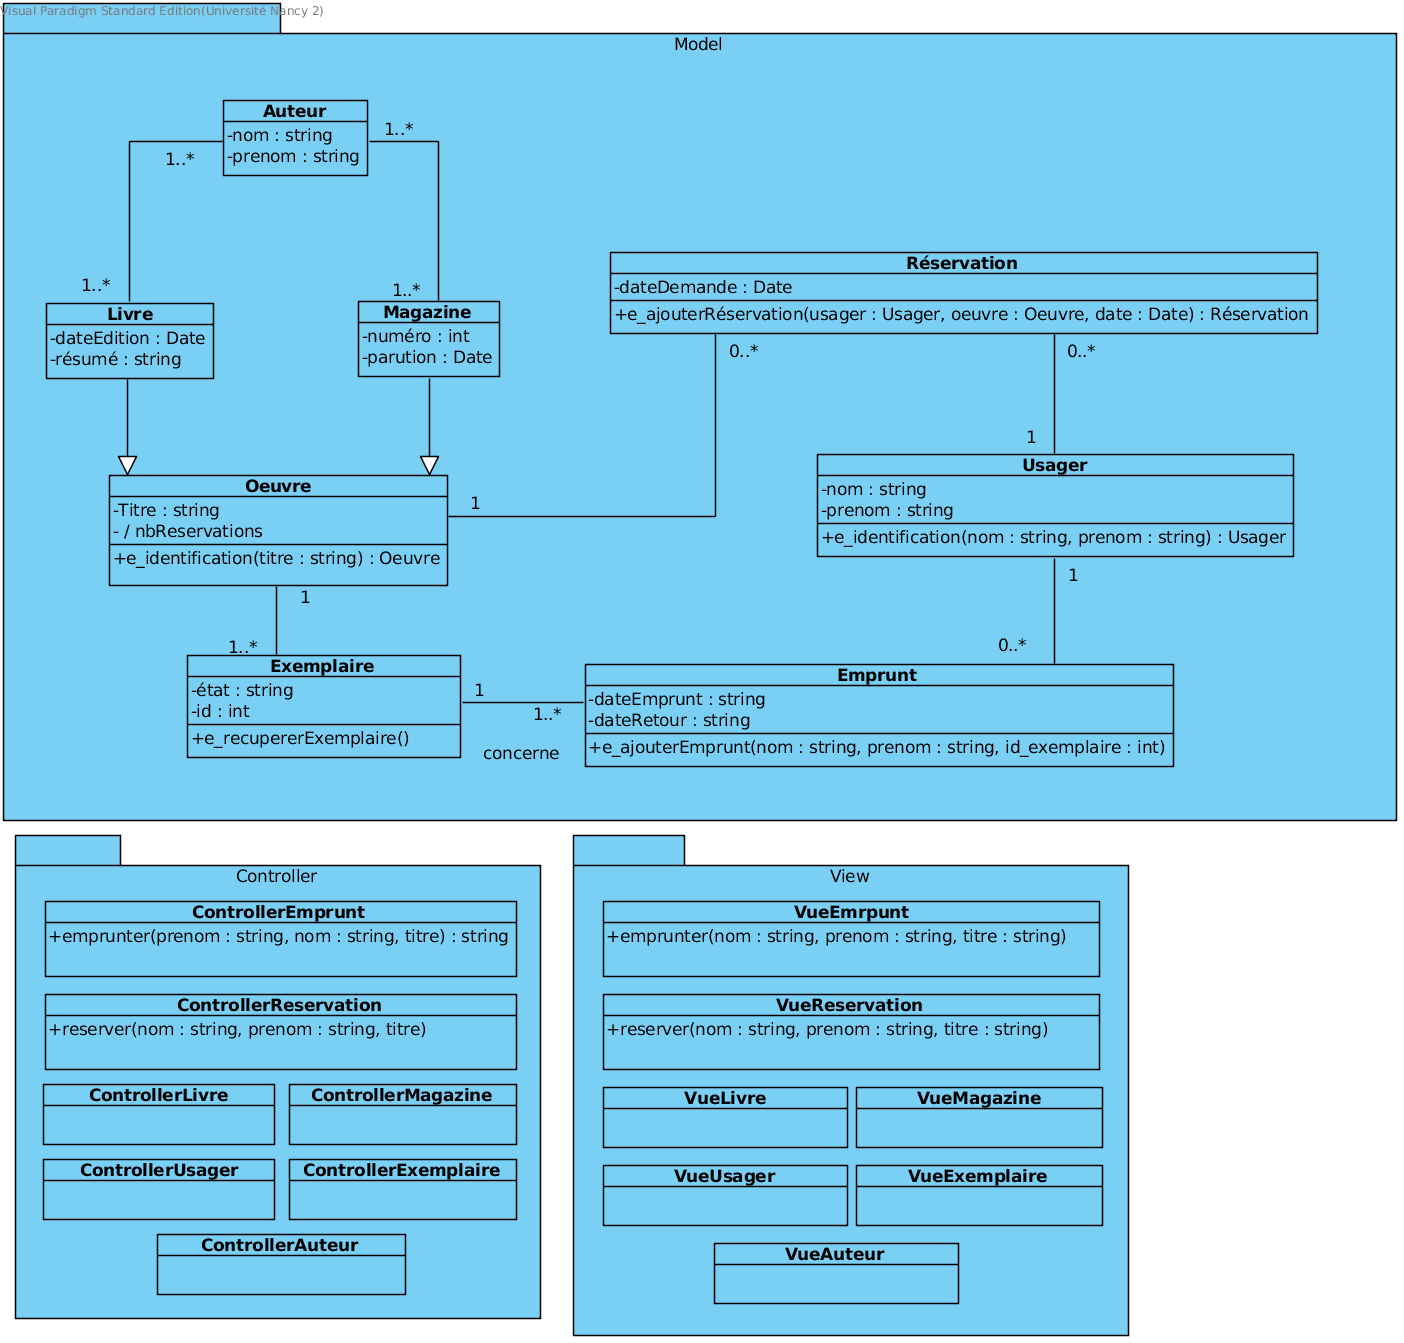
\includegraphics[width=.9\linewidth]{./res/img/diagramme-des-classes.png}
\caption{\label{fig:orgparagraph3}
Diagramme de classes}
\end{figure}



Nos objets métiers sont regroupés dans le paquetage \texttt{Model}. Il représente les
liaisons entre chaque entité. On peut par exemple voir qu’un Exemplaire est
associé à 1 ou plusieurs Emprunt(s).

Le paquetage \texttt{Controller} regroupe tout ce qui concerne la manipulation de ces
objets métiers. Les opérations basiques CRUD ne sont pas représentées car
elles sont présentes dans chaque entité.

Le paquetage \texttt{View} regroupe tout ce qui concerne l’Interface Homme Machine de
l’application. C’est avec les fonctions de ces entités que la bibliothécaire
va interagir.

\clearpage

\subsubsection{Diagramme d’états}
\label{sec:orgheadline8}

L’entité Œuvre a demandé l’utilisation d’un diagramme d’états pour décrire
comment le nombre de réservations d’une œuvre donnée va évoluer pendant
l’utilisation de l’application.


\begin{figure}[htb]
\centering
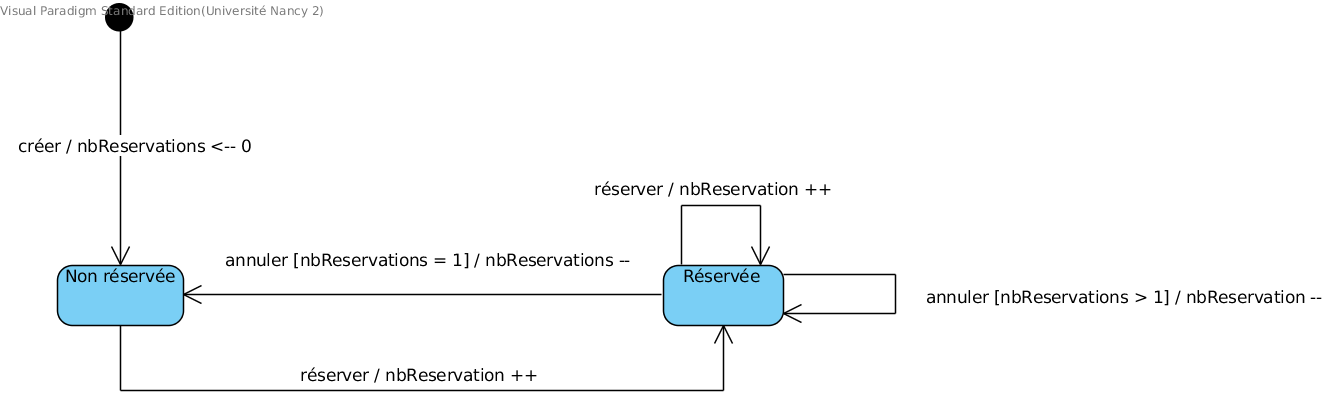
\includegraphics[width=.9\linewidth]{./res/img/oeuvre.png}
\caption{\label{fig:orgparagraph4}
État d'une œuvre}
\end{figure}


Une œuvre va passer par 2 états : \texttt{Non réservée} et \texttt{Réservée}. Lorsqu’une
nouvelle œuvre est ajoutée par la bibliothécaire, elle n’est pas réservée
par défaut (son nombre de réservations et donc de 0).
Un utilisateur réservant une œuvre induit une incrémentation du nombre de réservations de 1.
L’œuvre passe donc dans l’état \texttt{Réservée}.
Une annulation de réservation induit une décrémentation du nombre de réservations de 1.
Une fois le nombre de réservations à 0, l’œuvre repasse dans l’état \texttt{Non réservée}.

\subsubsection{Diagrammes de séquences}
\label{sec:orgheadline11}

Seuls les diagrammes de séquence des deux cas d’utilisation présentés vont être décrit ici.

\begin{enumerate}
\item Réserver une œuvre
\label{sec:orgheadline9}

\begin{figure}[htb]
\centering
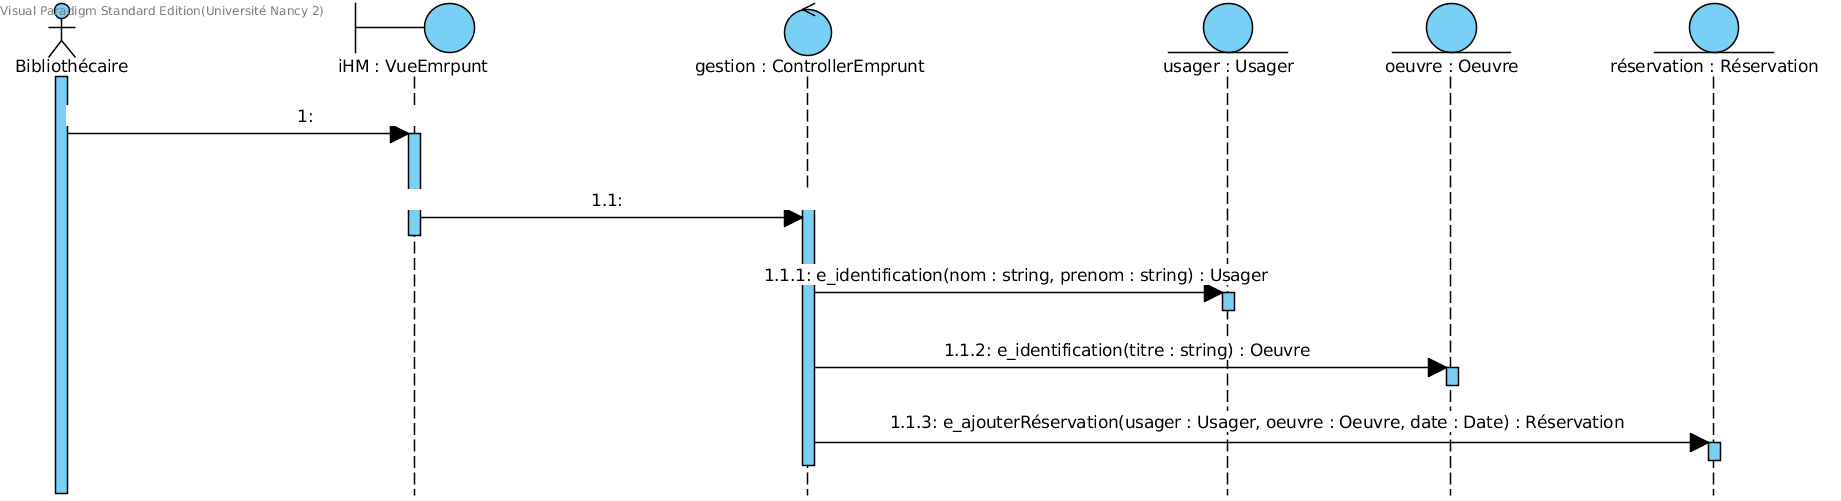
\includegraphics[width=.9\linewidth]{./res/img/reserver-oeuvre.png}
\caption{\label{fig:orgparagraph5}
Réserver une œuvre}
\end{figure}


Afin de créer une réservation pour une œuvre, la bibliothécaire va dans un
premier temps interagir avec l’IHM (une entité de notre paquetage \texttt{View} dans le
diagramme des classes) en renseignant les informations nécessaires (celles pour
permettre l’identification de l’Usager et de l’Œuvre). Cette IHM interagit avec
le contrôleur qui lui est associé (une entité du paquetage \texttt{Controller} du
diagramme des classes). Ainsi, il permet d’identifier l’usager grâce aux
informations remplies par la bibliothécaire. L’application va ensuite identifier
l’œuvre concernée. Pour finir, elle va créer une réservation concernant
l’œuvre identifiée pour l’usager identifié, en ajoutant la date du jour).

\item Emprunter un exemplaire d’une œuvre réservée
\label{sec:orgheadline10}

\begin{figure}[htb]
\centering
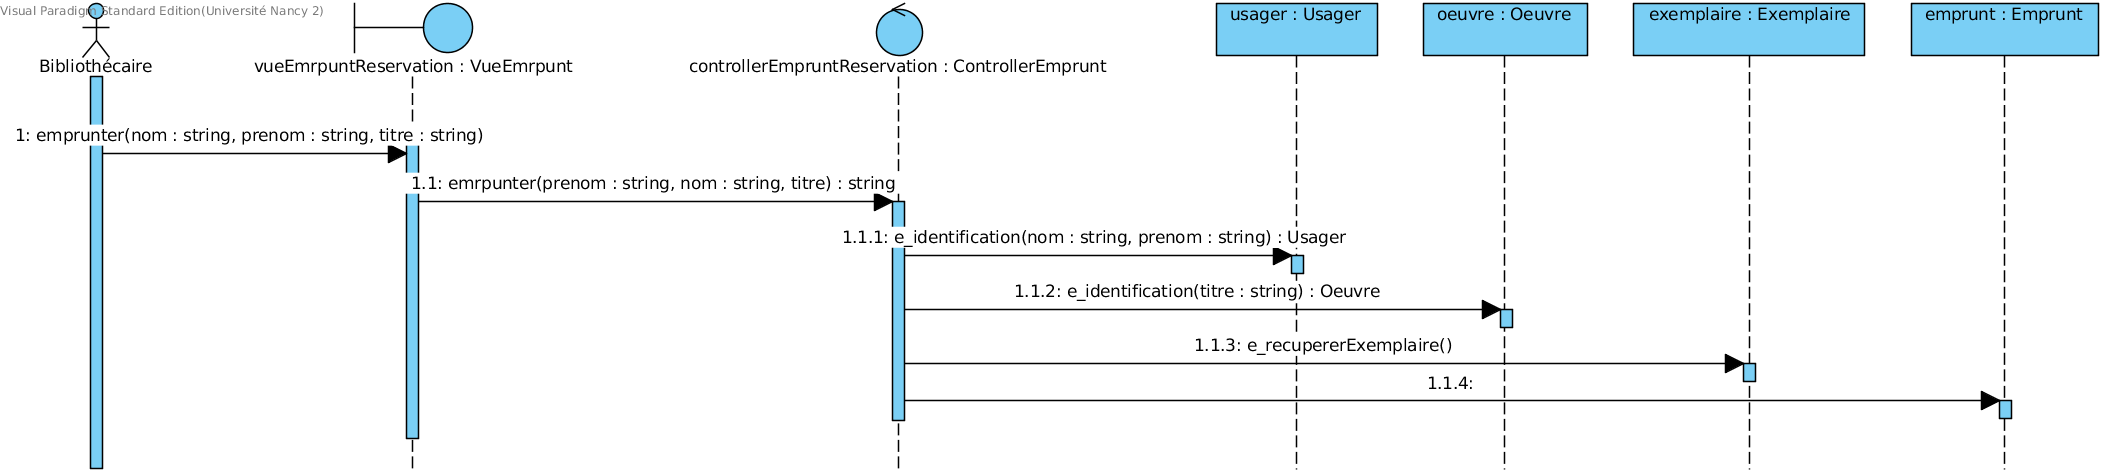
\includegraphics[width=.9\linewidth]{./res/img/emprunter-exemplaire1.png}
\caption{\label{fig:orgparagraph6}
Emprunter un exemplaire}
\end{figure}

Le principe est similaire au précédent diagramme.
La bibliothécaire interagit avec l’IHM pour renseigner les informations
nécessaires à l’identification de l’œuvre, de l’usager et de l’exemplaire.
Le contrôleur associé va interagir avec les objets métiers Usager, Œuvre,
Exemplaire et Réservation. Il va récupérer l’usager concerné par l’emprunt,
identifier l’œuvre, récupérer un exemplaire de cette œuvre. La réservation
de cet usager pour l’œuvre concernée et supprimée, et un nouvel emprunt est
créé.
\end{enumerate}



\subsection{Architecture de la solution}
\label{sec:orgheadline15}

\subsubsection{Diagramme de composants}
\label{sec:orgheadline13}

\begin{wrapfigure}[15]{r}{0.4\linewidth}
\vspace{-17pt}

\label{wrap-fig:emprunt-reserve}
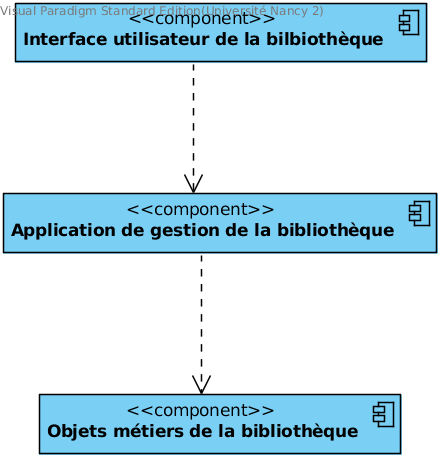
\includegraphics[width=\linewidth]{./res/img/ihm.png}
\end{wrapfigure}

Comme on a pu le voir dans le diagramme des classes, l’application se
découpe en trois couches qui interagissent entre elles. L’interface
utilisateur de la bibliothèque qui va permettre à la bibliothécaire
d’effectuer les actions exprimées dans le cahier des charges. L’application
de gestion, contient les entités qui vont interagir avec les objets métiers.
Les objets métiers de la bibliothèque qui sont la représentation physique
des données.

De cette description succincte des composants de l’application découle le
diagramme de déploiement, qui va permettre de définir l’architecture
applicative de la solution.


\subsubsection{Diagramme de déploiement}
\label{sec:orgheadline14}

\begin{figure}[htb]
\centering
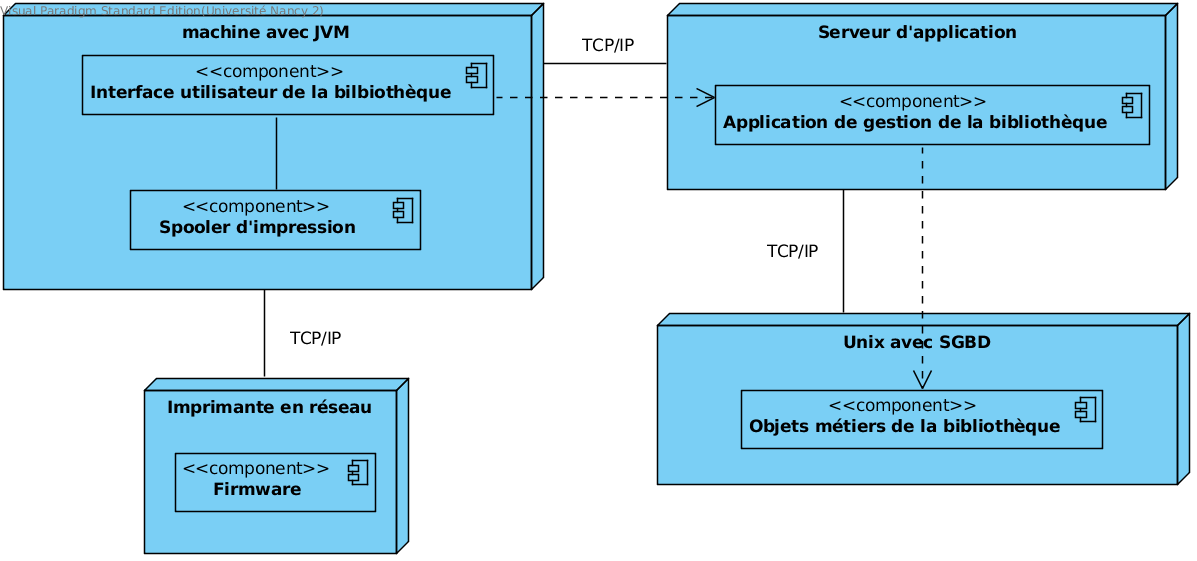
\includegraphics[width=.9\linewidth]{./res/img/diagramme-de-deploiement.png}
\caption{\label{fig:orgparagraph7}
Diagramme de déploiement}
\end{figure}

Ici dans un cadre d’application en production, les données physiques sont
stockées dans un SGBD. Il communique par protocole TCP/IP à l’application de
gestion de la bibliothèque contenue dans un serveur d’application sur une
machine avec une JVM.

\section{Implémentation}
\label{sec:orgheadline20}
\subsection{Particularités}
\label{sec:orgheadline17}

Comme vu sur le diagramme de composants, Bibal est une application distribuée composée de plusieurs tiers:
\begin{itemize}
\item une application web côté serveur,
\item une application web côté navigateur (faisant office d'IHM),
\item une base de données.
\end{itemize}

La base de données est une base relationnelle, aussi elle ne supporte pas
l’héritage. Livre et Magazine sont des spécialisations d’Œuvre Nous avons
donc construit un modèle physique des données pour modéliser les relations
entre Livre, Magazine et les entitées associées.

\begin{figure}[htb]
\centering
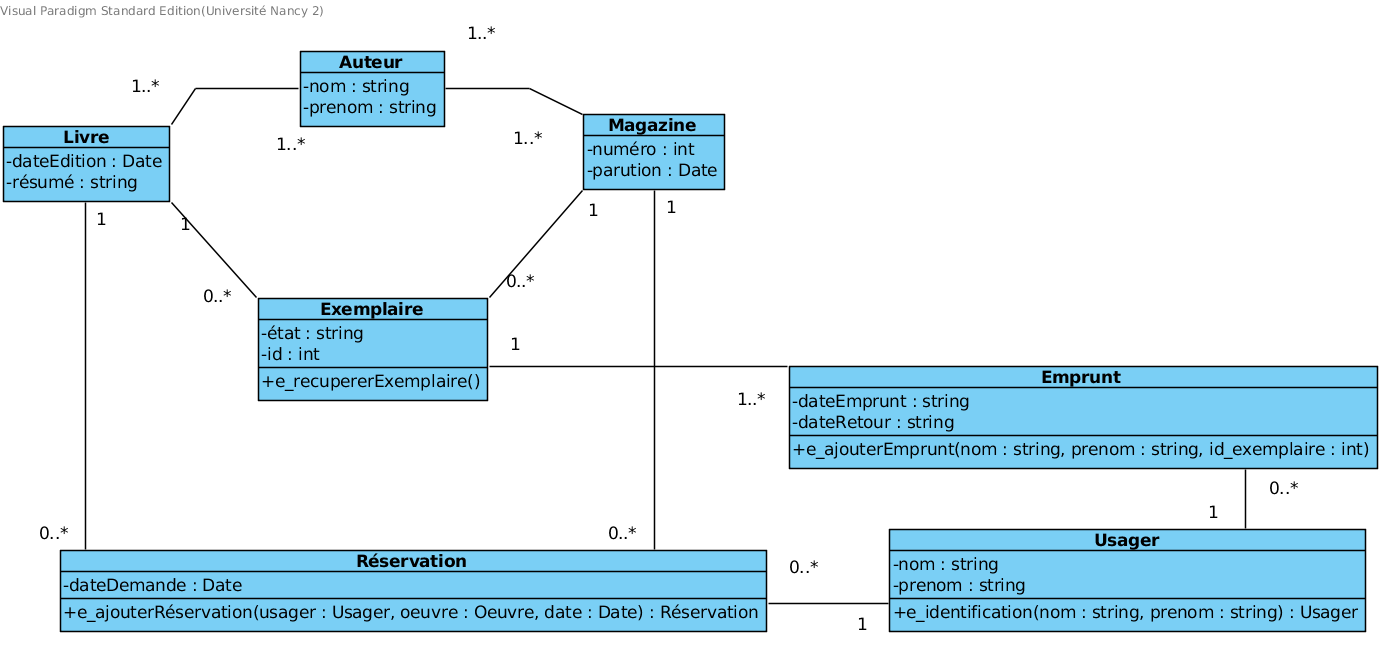
\includegraphics[width=.9\linewidth]{./res/img/mpd.png}
\caption{\label{fig:orgparagraph8}
Modèle physique des données}
\end{figure}


Nous avons également ajouté une fonctionnalité d’authentification. La
bibliothécaire étant la seule personne utilisant l’application, il nous
paraissait important que personne d’autre ne puisse gérer les usagers, les
réservations, etc.


Notre implémentation a été réalisée avec :
\begin{itemize}
\item MariaDB pour la base de données,
\item Hibernate pour gérer la persistance des données,
\item Spring Boot pour la logique applicative,
\item AngularJS pour l’interface homme-machine.
\end{itemize}



\clearpage

\subsection{Captures d’écran de l’application}
\label{sec:orgheadline18}

La page d’accueil de l’application permet plusieurs choses :
\begin{itemize}
\item enregistrer un utilisateur,
\item se connecter à l’application,
\item visualiser les livres et magazines présents dans la bibliothèque.
\end{itemize}



\begin{figure}[htb]
\centering
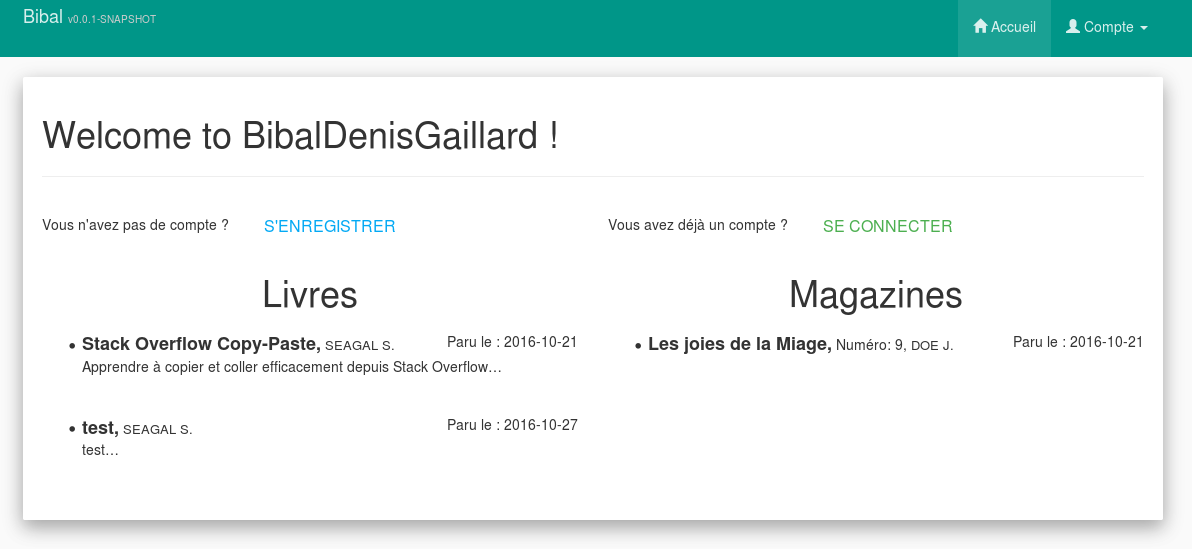
\includegraphics[width=.9\linewidth]{./res/img/screen-login.png}
\caption{\label{fig:orgparagraph9}
Page d'accueil}
\end{figure}

En tant que bibliothécaire connecté, d’autres fonctionnalités de gestion sont
débloquées pour les différents objets métiers. Les opérations CRUD sur tous
les objets sont possibles si l'on est identifié en tant que bibliothécaire.


\begin{figure}[htb]
\centering
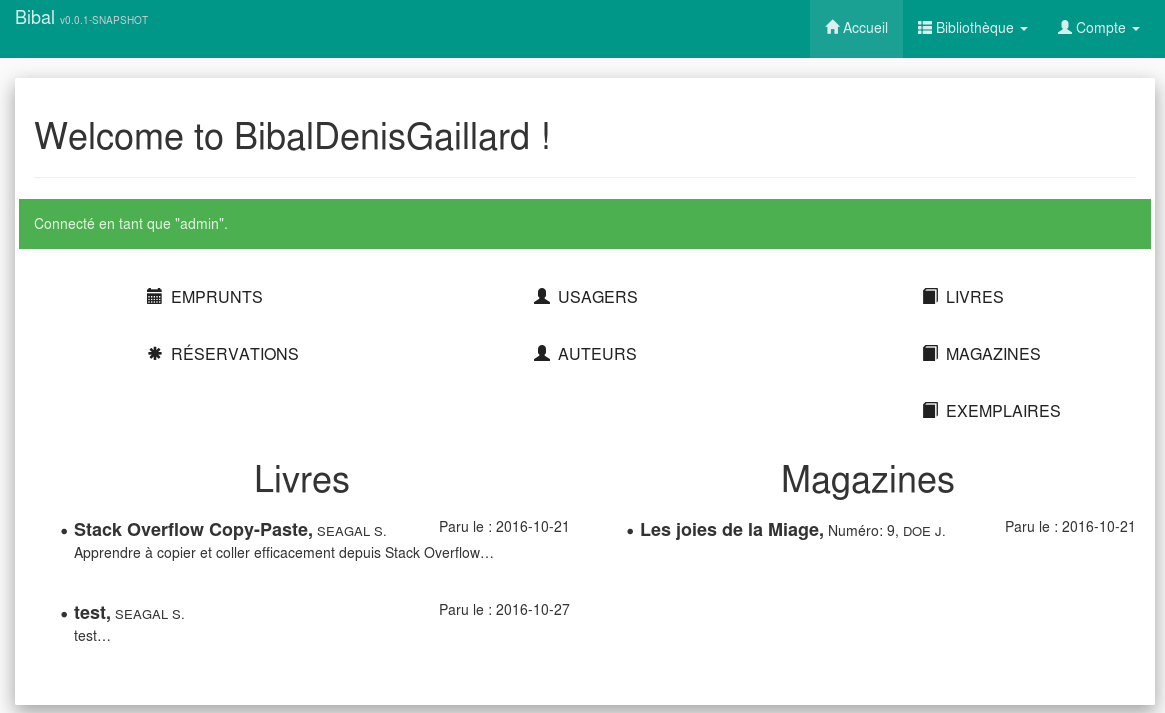
\includegraphics[width=.9\linewidth]{./res/img/screen-logged.png}
\caption{\label{fig:orgparagraph10}
Page d'accueil en étant authentifié}
\end{figure}


La vue des emprunts permet à la bibliothécaire, en plus des opérations CRUD,
de rendre l’exemplaire associé à cet emprunt.

\begin{figure}[htb]
\centering
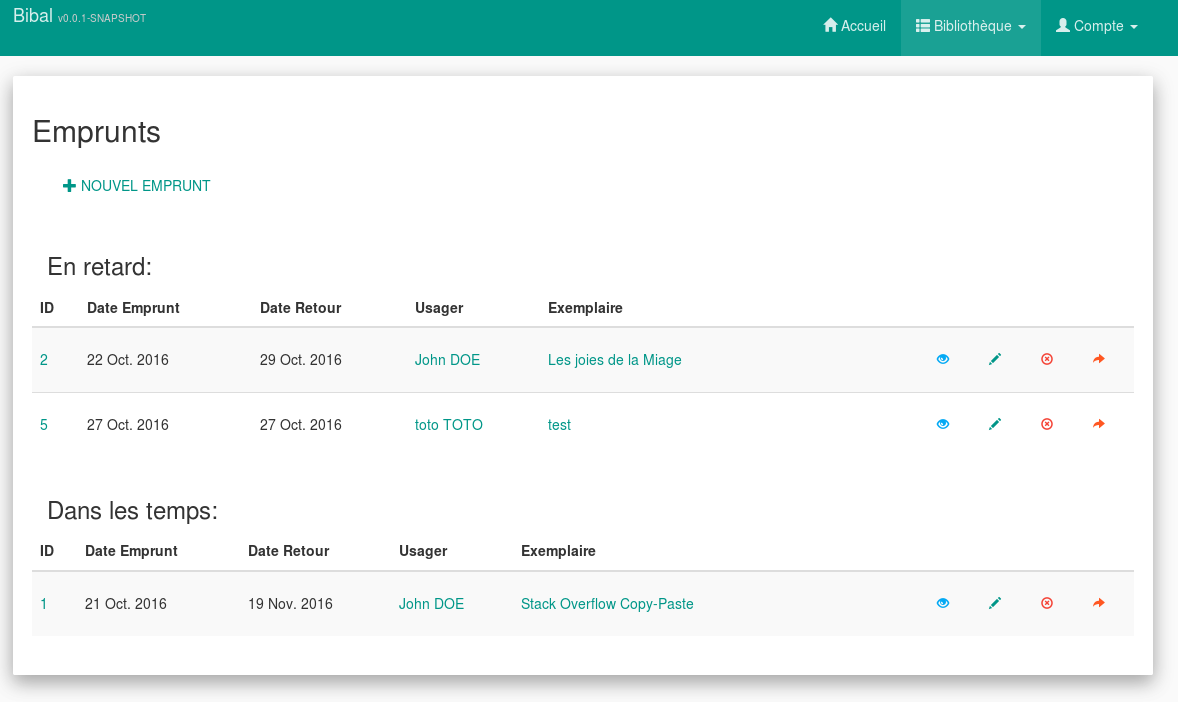
\includegraphics[width=.9\linewidth]{./res/img/screen-emprunt.png}
\caption{\label{fig:orgparagraph11}
Emprunts}
\end{figure}


\subsection{Résumé}
\label{sec:orgheadline19}

Toute la difficulté de cette réalisation réside dans la compréhension du
besoin et des contraintes, de leurs raisons d’être et de comment réaliser la
solution en en tenant compte. L’adoption d’une démarche scientifique est
essentielle pour éviter les écueils classiques en matière de communication,
d’analyse, d’implémentation, de gestion des ressources (humaine, temporelles,
financières, etc\ldots{}). Nous avons décortiqué la problématique autant que
possible en étapes simples et tenté d’écarter au maximum toute ambiguïté. Le
résultat est simple mais répond au besoin : une application de gestion de
bibliothèque fournissant toutes les fonctionnalités demandées de façon
cohérente, simple d’accès, sécurisée, simple d’utilisation et facilement
évolutive.


\clearpage
\section{Annexes}
\label{sec:orgheadline30}
\subsection{Diagrammes d’activité}
\label{sec:orgheadline29}
\subsubsection{Créer un exemplaire}
\label{sec:orgheadline21}

\begin{figure}[!htpb]
\centering
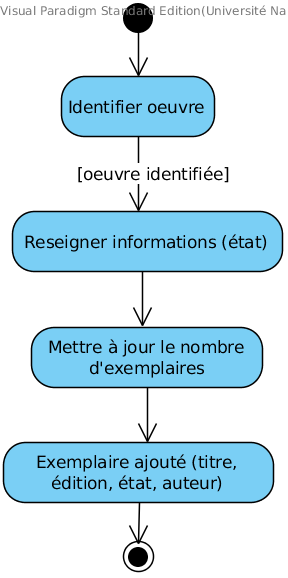
\includegraphics[width=5cm]{./res/img/ajouter-un-exemplaire.png}
\caption{\label{fig:orgparagraph12}
Créer un exemplaire}
\end{figure}


\clearpage
\subsubsection{Ajouter un usager}
\label{sec:orgheadline22}

\begin{figure}[!htpb]
\centering
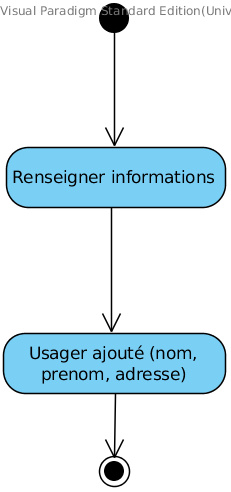
\includegraphics[width=5cm]{./res/img/ajouter-usager.png}
\caption{\label{fig:orgparagraph13}
Ajouter un usager}
\end{figure}

\clearpage
\subsubsection{Annuler une réservation}
\label{sec:orgheadline23}

\begin{figure}[!htpb]
\centering
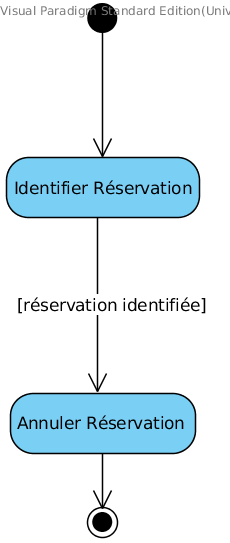
\includegraphics[width=5cm]{./res/img/annuler-reservation.png}
\caption{\label{fig:orgparagraph14}
Annuler une réservation}
\end{figure}


\clearpage
\subsubsection{Emprunter un exemplaire}
\label{sec:orgheadline24}

\begin{figure}[!htpb]
\centering
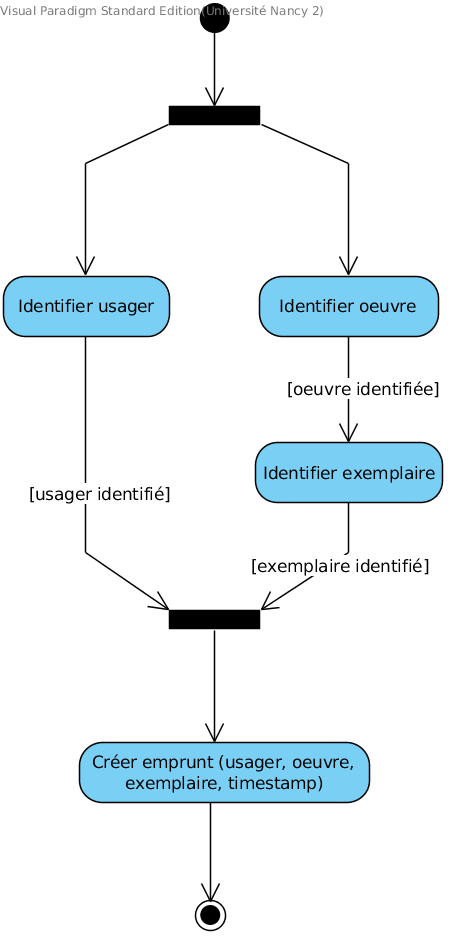
\includegraphics[width=5cm]{./res/img/emprunter-exemplaire.png}
\caption{\label{fig:orgparagraph15}
Emprunter un exemplaire}
\end{figure}

\clearpage
\subsubsection{Modifier un exemplaire}
\label{sec:orgheadline25}

\begin{figure}[!htpb]
\centering
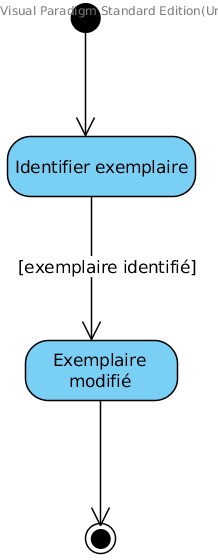
\includegraphics[width=5cm]{./res/img/modifier-exemplaire.png}
\caption{\label{fig:orgparagraph16}
Modifier un exemplaire}
\end{figure}


\clearpage
\subsubsection{Supprimer un exemplaire}
\label{sec:orgheadline26}

\begin{figure}[!htpb]
\centering
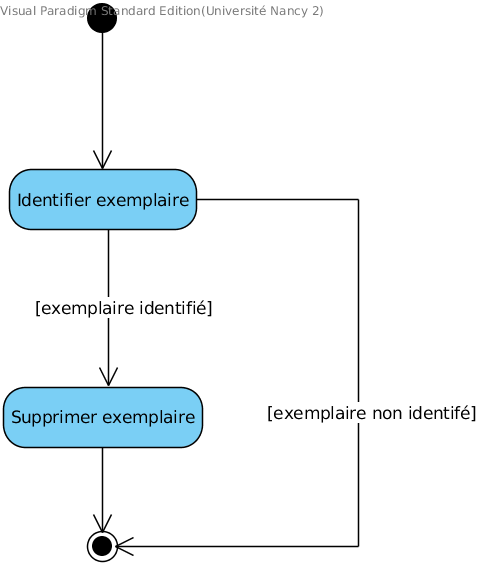
\includegraphics[width=10cm]{./res/img/supprimer-exemplaire.png}
\caption{\label{fig:orgparagraph17}
Supprimer un exemplaire}
\end{figure}

\clearpage
\subsubsection{Vérifier l’état d’un exemplaire}
\label{sec:orgheadline27}

\begin{figure}[htb]
\centering
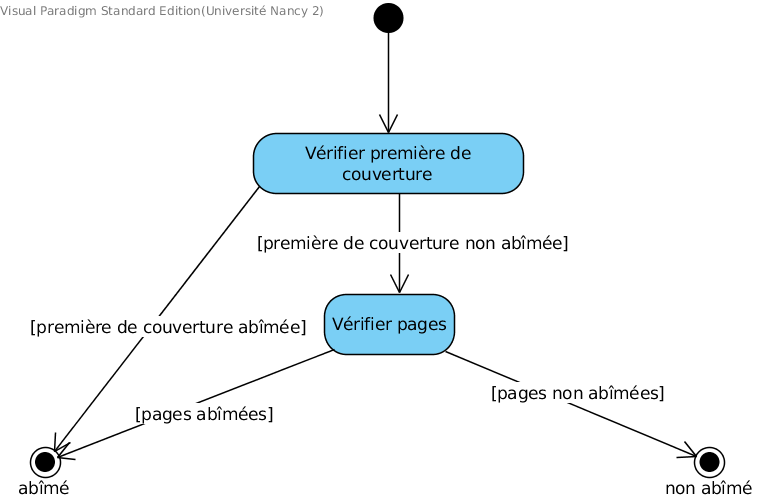
\includegraphics[width=.9\linewidth]{./res/img/verifier-etat-exemplaire.png}
\caption{\label{fig:orgparagraph18}
Vérifier l’état d’un exemplaire}
\end{figure}

\clearpage
\subsubsection{Rendre un exemplaire}
\label{sec:orgheadline28}

\begin{figure}[htb]
\centering
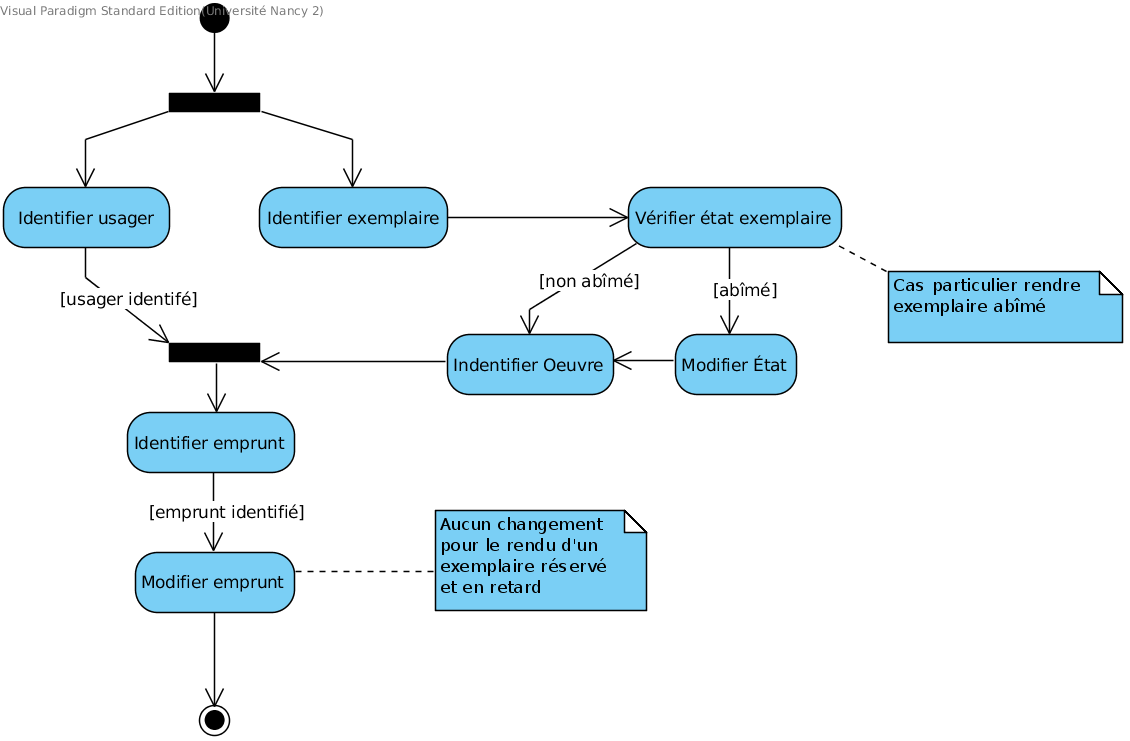
\includegraphics[width=.9\linewidth]{./res/img/rendre-un-exemplaire.png}
\caption{\label{fig:orgparagraph19}
Rendre un exemplaire}
\end{figure}
\end{document}
